\problemname{Investigating Frog Behaviour\\on Lily Pad Patterns}

\newcommand{\frogsprotagonist}{Ina}

\illustration{0.32}{illustration}{A frog in a pond.\vspace{-0.5cm}}%
Recently, the biologist \frogsprotagonist{} discovered a new frog species
on the lily pads of a pond.
She observed the frogs for a while and found them to be very conscious
about their personal space because they avoided sharing a lily pad with other frogs.
Also, they seemed quite lazy as they did not move often, and if they did,
they always jumped to the nearest empty lily pad.

To confirm her hypotheses about the frogs' movement pattern, \frogsprotagonist{} set up
a large number of lily pads in a pool in her laboratory, arranged in a straight line.
Since the frogs were attracted to light, she was able to simplify the test setup
further by placing a bright light at one end of that line. This way, the frogs
would always jump in one direction (towards the light).

Of course, \frogsprotagonist{} could now place some frogs on the lily pads and
sit there all day watching the frogs jump around. But as the frogs
move so rarely, it would take ages to gather a sufficient amount of data.

She therefore attached to each frog a tiny device that could log all jumps of that frog.
This way, she could put the frogs on the lily pads, leave
them alone for a few hours and come back later to collect the data.
Unfortunately, the devices had to be so tiny that there was no space
for a position tracking system; instead, the devices could only record the times of the jumps.

But if the movement pattern of the frogs is as restricted as \frogsprotagonist{} thinks, surely the
individual movements of the frog can be reconstructed only from the initial positions and
the recorded jump time stamps?

\begin{Input}
	The input consists of:
	\begin{itemize}
		\item One line with an integer $n$ ($1\leq n \leq 2\cdot10^5$), the number of frogs.
		\item One line with $n$ integers $x_1,\dots, x_n$ ($1\leq x_i \leq 10^6$),
			the number of the lily pad on which the $i$th frog initially sits.
			The lily pads are numbered consecutively, starting at $1$. 
			It is guaranteed that the initial positions are strictly increasing, i.e.\
			$x_1 < x_2 < \dots < x_n$.
		\item One line with an integer $q$ ($1\leq q \leq 2\cdot10^5$), the
			number of jumps recorded.
		\item $q$ lines, each containing an integer $i$ ($1\leq i\leq n$), indicating
			that the $i$th frog jumped. The jumps are given in chronological
			order and you may assume that a jumping frog lands before the next
			jump begins.
			The frogs always jump to the nearest empty lily pad with a larger number,
			and you may assume that such a lily pad always exists.
	\end{itemize}
\end{Input}

\begin{Output}
	For each jump, output the number of the lily pad the frog lands on.
\end{Output}

\begin{afterSample}
  \section*{Notes}
	\begin{figure}[h]
		\centering
		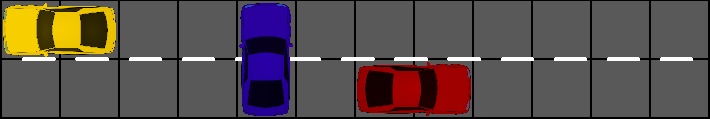
\includegraphics[width=\textwidth]{sample}
		%\vspace{3mm}
		\caption{Illustration of the first sample case. The lily pads are
		numbered from left to right, starting at $1$.}
	\end{figure}
\end{afterSample}
